%!TEX root = ../talk.tex

\section{Caffe}\label{sec:Caffe}

%%%

\frameinlbffalse

{
\usebackgroundtemplate{
\tikz[overlay,remember picture] \node[opacity=0.8, xshift=-3cm, at=(current page.east)] {
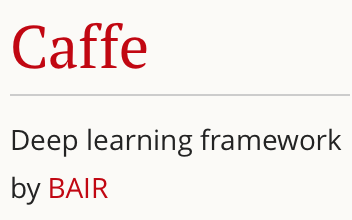
\includegraphics[width=0.3\paperwidth]{figures/Caffe_logo.png}
};}

\begin{frame}[plain]
\frametitle{\S\ref{sec:Caffe}. \insertsection}
\listofframes
\end{frame}
\addtocounter{framenumber}{-1} % this page does not count

}

\frameinlbftrue

%%%
\subsection{Programming interface}
%%%

\begin{frame}
  \MyLogo
  \frametitle{General Comments}  

\begin{enumerate}\setlength\itemsep{0.6em}
%
\item Mainly focus on (and well suited for) CNN and image recognition 
\begin{itemize}
\item Use an expressive architecture
\item Provide simple command line tools for training and prediction
\item Allow defining models and optimization by configuration
\item Use Google protocol tool to define parameters for nets and solvers
\end{itemize}
%
\item Not so convenient to extend 
\begin{itemize}
\item Write layers in C++ or Python, handwritten CUDA code
\item Not well documented
\item No automatic differentiation
\item Not as flexible as other engines
\item Python interface not transparent
\end{itemize}
%
\item Lots of dependencies; can be tricky to install
%
\end{enumerate}

\end{frame}

%%%
\subsection{Simple examples}
%%%
\begin{frame}[fragile]
  \MyLogo
  \frametitle{Example: Image Classification}  

\begin{lstlisting}[language=python]
import caffe
import matplotlib.pyplot as plt

# paste your image URL here
my_image_url = "https://wikipedia/Orang_Utan/2C_Malaysia.JPG"
!wget -O image.jpg $my_image_url

# transform it and copy it into the net
image = caffe.io.load_image('image.jpg')
caffe.net.blobs['data'].data[...]=transformer.preprocess('data',image)

# perform classification
caffe.net.forward()

# obtain the output probabilities
output_prob = net.blobs['prob'].data[0]

# sort top five predictions from softmax output
top_inds = output_prob.argsort()[::-1][:5]

# 
plt.imshow(image)

#
print 'probabilities and labels:'
zip(output_prob[top_inds], labels[top_inds])
\end{lstlisting}

\vskip 50pt

\end{frame}

%%%

\begin{frame}[fragile]
  \MyLogo
  \frametitle{Example: Extend Layers}  
\begin{lstlisting}[language=python]
import caffe
import numpy as np 

class EuclideanLoss(caffe.layer):
	def setup(self, bottom, top):
		if len(bottom) != 2: #check number of input data
			raise Exception("Need two inputs to compute distance")
			
	def reshape(self, bottom, top):
		#check input dimensions match
		if bottom[0].count != bottom[1].count:
			raise Exception("Inputs must have the same dimension")
		#difference in shape of inputs
		self.diff = np.zeros_like(bottom[0].data, dtype=np.float32)
		# loss output is scalar
		top[0].reshape(1)
		
	def forward(self, bottom, top):
		self.diff[...] = bottom[0].data - bottom[1].data
		top[0].data[...] = np.sum(self.diff**2)/bottom[0].num/2.	

	def backward(self, top, propagate_down, bottom):
		for i in range(2):
			if not propagate_down[i]:
				continue
			if i == 0:
				sign = 1
			else:
				sign = -1
			bottom[i].diff[...] = sign.self.diff / bottom[1].num
\end{lstlisting}
\end{frame}

%%%

\begin{frame}[fragile]
  \MyLogo
  \frametitle{Example: Extend Layers (Cont)}  
  
\ContinueLineNumber
\structure{Define a class in Python to extend Layer}
\begin{lstlisting}[language=python]
layer{
	type: "Python"
	python_param {
		module: "laylers"
		layer: "EuclideanLoss"
	}
}
\end{lstlisting}

\vskip 110pt

\tiny
\begin{center}
{
\color{red}https://docs.google.com/presentation/d/1UeKXVgRvvxg9OUdh\_UiC5G71UMscNPlvArsWER41PsU/edit\#slide=id.gc2fcdcce7\_216\_0
}
\end{center}
\end{frame}